% This file was created by tikzplotlib v0.8.5.
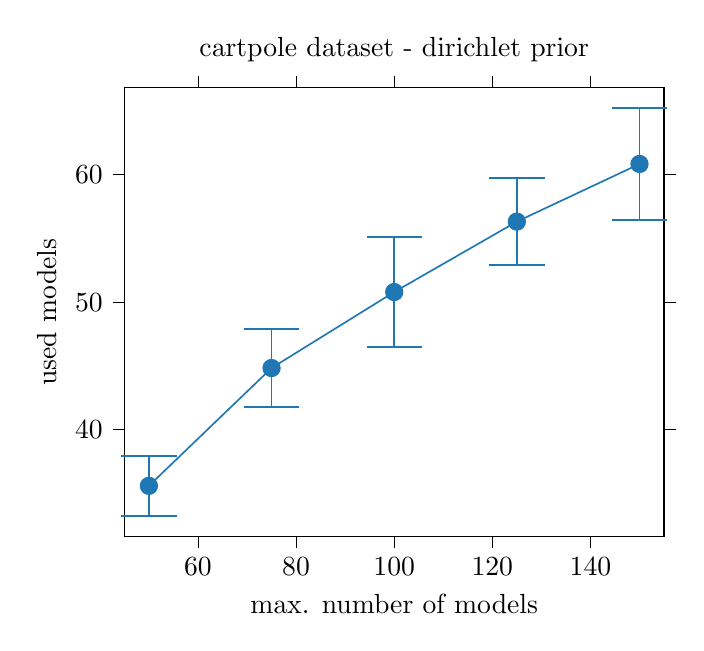
\begin{tikzpicture}

\definecolor{color0}{rgb}{0.12156862745098,0.466666666666667,0.705882352941177}

\begin{axis}[
tick align=outside,
tick pos=both,
title={cartpole dataset - dirichlet prior },
x grid style={white!69.01960784313725!black},
xlabel={max. number of models},
xmin=45, xmax=155,
xtick style={color=black},
y grid style={white!69.01960784313725!black},
ylabel={used models},
ymin=31.6525728763888, ymax=66.8076730481651,
ytick style={color=black}
]
\path [draw=color0, semithick]
(axis cs:50,33.2505319751059)
--(axis cs:50,37.9494680248941);

\path [draw=color0, semithick]
(axis cs:75,41.797895465307)
--(axis cs:75,47.882104534693);

\path [draw=color0, semithick]
(axis cs:100,46.4825933710154)
--(axis cs:100,55.1174066289846);

\path [draw=color0, semithick]
(axis cs:125,52.9056772267403)
--(axis cs:125,59.7343227732597);

\path [draw=color0, semithick]
(axis cs:150,56.4702860505521)
--(axis cs:150,65.209713949448);

\addplot [semithick, color0, mark=-, mark size=10, mark options={solid}, only marks]
table {%
50 33.2505319751059
75 41.797895465307
100 46.4825933710154
125 52.9056772267403
150 56.4702860505521
};
\addplot [semithick, color0, mark=-, mark size=10, mark options={solid}, only marks]
table {%
50 37.9494680248941
75 47.882104534693
100 55.1174066289846
125 59.7343227732597
150 65.209713949448
};
\addplot [semithick, color0, mark=*, mark size=3, mark options={solid}]
table {%
50 35.6
75 44.84
100 50.8
125 56.32
150 60.84
};
\end{axis}

\end{tikzpicture}
